%!TEX root = ../../dissertation.tex
%%%%%%%%%%%%%%%%%%%%%%%%%%%%%%%%%%%%%%%%%%%%%%%%%%%%%%%%%%%%%%%%%%%%%%%%%%%%%%%%
\section{Dataset and Methodology}
\label{c4:sec:methodology}

For our analysis, we use the \gls{METAWIN} monitoring system developed in a previous research project and deployed in the network of an Austrian mobile operator.  More in-depth information about \gls{METAWIN} is available in \cite{ricciato_2011}.

 The location of the measurement probe at the Gn interface within the core network, marked in Figure~\ref{c4:fig:umtsnetwork}, gives access to both wide-area mobility signaling (not analyzed in this paper) and signaling related to user-plane IP traffic (which we want to scrutinize). The \gls{METAWIN} monitoring system extracts and correlates information from the lower layers of the \gls{3GPP} protocol stack, and specifically the \gls{GTP} protocol on the Gn interface \cite{3gpp129.060}. This includes the \acrfull{RAT} identifier as well as the terminal types of the mobile clients. The latter is determinable by the \acrfull{TAC} part of the \acrfull{IMEI} (cf.~\cite{3gpp23.003}) and will be discussed later in detail.

To meet privacy requirements, the \gls{METAWIN} system anonymizes captured data on the fly at multiple layers: the application-level payload is removed and all user identifiers (e.g. \gls{IMSI}) are hashed with a one-way function before recording. That is, single \glspl{MS} in our dataset may be differentiated by means of an anonymized \gls{MS-ID}, but not traced back to the actual customer. The packet capturing hardware deployed within the \gls{METAWIN} monitoring system is synchronized using \gls{GPS}. Accordingly, the packet timestamps have an accuracy of $\pm100$ ns or better~\cite[p.97-98]{donnelly_high_2002}.



%%%%%%%%%%%%%%%%%%%%%%%%%%%%%%%%%%%%%%%%%%%%%%%%%%%%%%%%%%%%%%%%%%%%%%%%%%%%%%%%
\subsection{Network and Monitoring Setup}


%\begin{figure*}%[tbp]
%\centering
%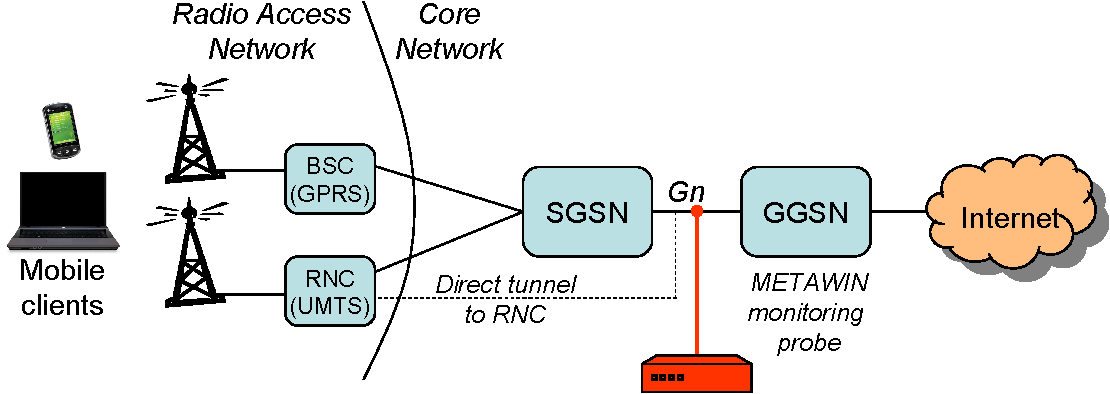
\includegraphics[width=0.98\textwidth]{figures/network_setup_gtp_tun-crop.pdf}
%\caption{Measurement setup.}
%\label{fig:net_setup}
%\end{figure*}

For our analysis, we use the \gls{METAWIN} monitoring system developed in a previous research project
and deployed in the network of an Austrian mobile operator.  More in-depth information about \gls{METAWIN} is available in \cite{ricciato_2011}.
The location of the measurement probe within the core network is highlighted in Figure~\ref{c4:fig:umtsnetwork}. 

As said before, the \gls{GGSN} acts as the IP-layer gateway for the user traffic. It is in charge of setting up,
maintaining, and tearing down a logical connection to each active \gls{MS}. This logical connection, the \gls{PDP} context,
is conceptually similar to a dial-up connection. During set up, an
IP address is dynamically assigned to the \gls{MS}.
%The \glspl{SGSN} and \glspl{GGSN} in the core network are interconnected by a wide-area IP network that
%will be referred to as the ``G$_n$ network'' following the terminology of \gls{3GPP} specifications
%(``Gn interface'').
In the network under study, a so-called \textit{direct tunnel} setup might be used for \glspl{MS} connected
via \gls{UMTS}/\gls{HSPA}. Such a setup consists of a direct link between \glspl{GGSN} and the
\glspl{RNC} %(indicated by the upper dashed line in Fig.~\ref{fig:umtsnetwork}), % Dashing is indiscernible in the figure.
which is used for
transporting user-plane data traffic only. Since signaling procedures such
as mobility management are carried out by the \glspl{SGSN}, a \gls{GGSN} always has to send signaling packets
via the path involving the \glspl{SGSN}. Monitoring the Gn interface thus gives us access to both wide-area mobility signaling (not analyzed in this paper) % routing area updates
and signaling related to user-plane IP traffic (which we want to scrutinize).
For more information on the \gls{3G} network structure, please refer to~\cite{bannister_convergence_2004}.

The METAWIN monitoring system extracts and correlates information from the lower
layers of the \gls{3GPP} protocol stack, and specifically the \gls{GTP} protocol
on the Gn interface \cite{3gpp129.060}. This includes the \acrfull{RAT} identifier as well as the terminal types of the mobile clients. The
latter is determinable by the \acrfull{TAC} part of the \acrfull{IMEI} (cf. \cite{3gpp23.003}) and will be discussed later in detail.

To meet privacy requirements, the METAWIN system anonymizes captured data on the fly at multiple
layers: the application-level payload is removed and all user identifiers (e.g. \gls{IMSI}) are
hashed with a one-way function before recording. That is, single
\glspl{MS} in our dataset may be differentiated by means of an anonymized \gls{MS-ID}, but not traced back to the actual customer.
The packet capturing hardware deployed within the METAWIN monitoring system is synchronized
using \gls{GPS}. Accordingly, the packet timestamps
have an accuracy of $\pm100$ ns or better~\cite[p.97-98]{donnelly_high_2002}.



%%%%%%%%%%%%%%%%%%%%%%%%%%%%%%%%%%%%%%%%%%%%%%%%%%%%%%%%%%%%%%%%%%%%%%%%%%%%%%%%
\subsection{Dataset Description}

% TODO: more detailed data set description? maybe table? (# of entries etc)

%TODO: OLD
The \gls{METAWIN}-recorded dataset used in our evaluation is a week-long trace from the third week of April 2011. It consists of 2.2 billion aggregated flows for the user traffic and 410 million \gls{GTP} Tunnel Management transactions, the latter representing the data base for this paper. It was tapped at one of the \glspl{GGSN} of the operator, and contains about half of the total traffic volume handled by the operator in this period. The \gls{GTP} data contains the response codes for each transactions. With these codes, failed interactions can be sorted out and treated separately.

We fed the records into a SQL database, and conducted further evaluations through scripted queries on the database. Any privacy-relevant data, e.g. the \gls{IMEI}, \gls{MS-ID} and any IP address involved, is only visible as hashes and is processed in a privacy-preserving manner.  Since the hashing of the \gls{IMEI} is consistent throughout the dataset, user traffic flows and the \gls{GTP} data can be cross-correlated despite anonymization, giving the opportunity for further research.


%%%%%%%%%%%%%%%%%%%%%%%%%%%%%%%%%%%%%%%%%%%%%%%%%%%%%%%%%%%%%%%%%%%%%%%%%%%%%%%
\subsection{Device Identification \& Classification}

Individual device types can also still be identified in form of the \gls{TAC} on every entry. The \gls{TAC} is part of the \gls{IMEI}, uniquely identifying each device type \cite{3gpp23.003}. The rest of the \gls{IMEI} constitutes the serial number of the involved devices, which is not present in the data.

\glspl{TAC} are managed by the GSM Association which in turn assigns local organizations, distinguished by the first two digits of the \gls{TAC} as Reporting Body Identifier, to allocate \glspl{TAC} to manufacturers. However, this allocation information is not freely available. Commercial databases exist, but this is neither affordable for research institutions, nor is it conducive to our goal of providing information to the public. While there are some websites that allow one to query for specific \glspl{TAC} for non-commercial purposes, only very few efforts attempt to collect \gls{TAC} information into a publicly available database. We based our data-mining efforts on a publicly available set\footnote{\url{http://www.mulliner.org/tacdb/}, Mulliner, C.}, with some additional devices collected on our own. Since the unit identification part of the \gls{IMEI} is just six decimal digits long, popular devices will even be assigned more than one TAC, making the acquisition of all relevant \glspl{TAC} even more complicated.

For our investigation, we went through large portions of the \glspl{TAC} present in our dataset, and identified and categorized the most important entries. In this case, importance means various metrics like the traffic volume, the number of flows, and the number of \gls{GTP} signaling messages for each \gls{TAC}. 

After having available the device names for most \glspl{TAC}, we were able to add meta-information and categorize the entries based on their device type and operating system. For the device type we partitioned the devices roughly into smartphones, regular mobile phones and 3G USB dongles or 3G/WiFi routers. The operating system includes most of the popular incarnations found in the network at measurement time, including Android, iOS, and Symbian. Note however that many devices, especially USB dongles cannot be linked to any specific OS.

\begin{table}
\centering
\caption{Relative \acrshort{TAC} Statistics.}
\label{c4:tbl:tacstats}
\begin{tabu}{|l|X[r]|}
\hline
& \textbf{Portion of devices with entry in TAC DB}\\ \hline
\# of Flows & 99.72\% \\
Ratio of Traffic & 99.97\%\\
\# of Tunnels & 87.57\% \\
\# of GTP Signaling Msgs & 90.95\% \\
\# of Distinct \glspl{MS-ID} & 80.93\%\\ \hline
\end{tabu}
\end{table}

As we are working with an incomplete \gls{TAC} database it is important to know whether our \gls{TAC} mappings provide sufficiently useful data to allow for the envisioned device discriminating statistics. Therefore, Table~\ref{c4:tbl:tacstats} provides some statistics on our knowledge of devices in the dataset. About 80 percent of all distinct and active devices could be identified. Looking at the total number of \gls{GTP} signaling messages, we see that we can determine the device name of over 90 percent. The flow data shows an even clearer picture, as we can identify almost all of the devices involved.

After applying the categorization to the \glspl{TAC} we evaluate the device composition in the network. The two largest portions of devices are smartphones and 3G dongles, while classic cell phones do not seem to play a major role in the packet-switched domain anymore. One observation across all device types is that about 14 percent of all mobile devices have activated their mobile data service and have signaling traffic, but do not cause any user plane traffic.

The difference between 3G dongles and smartphones is also noteworthy. While the former cause large amounts of user plane traffic (compared to the device numbers), they are responsible for but a few core network signaling events and tunnels. This picture is reversed for smartphones.


%%%%%%%%%%%%%%%%%%%%%%%%%%%%%%%%%%%%%%%%%%%%%%%%%%%%%%%%%%%%%%%%%%%%%%%%%%%%%%%%


In this section we attempt to shed some light on the overall control plane dynamics in a mobile core network. We evaluate a dataset recorded in a live 3G network for PDP Context durations, and attempt to show the possible impact of certain device categories on the total tunnel durations. As discussed before, this can serve as a proxy metric for the signaling load on the system. 


%%%%%%%%%%%%%%%%%%%%%%%%%%%%%%%%%%%%%%%%%%%%%%%%%%%%%%%%%%%%%%%%%%%%%%%%%%%%%%%%
\subsection{Dataset Description}
Our dataset, kindly provided by an Austrian mobile operator and recorded using the \gls{METAWIN} monitoring system, was taken in the third week of April 2011. It consists of seven days of aggregated flow-level data for the user traffic and a summary entry for every \gls{GTP} Tunnel Management transaction, the latter representing the data base for this paper. It was tapped at one of the \glspl{GGSN} of the operator, and contains about half of the total traffic volume handled by the operator in this period. The \gls{GTP} data contain the response codes for each transactions. With these codes, failed interactions can be sorted out and treated separately.

We fed the records into a SQL database, and conducted further evaluations through scripted queries on the database. Any privacy-relevant data, e.g. the \gls{IMEI}, \gls{MS-ID} and any IP address involved, is only visible as hashes and can only be processed in anonymized form. Individual device types can be identified in form of the unhashed \gls{TAC} on every entry. Since the hashing of the \gls{IMEI} is consistent, user traffic flows and the \gls{GTP} data can be cross-correlated despite anonymization, giving the opportunity for further research.

 

%%%%%%%%%%%%%%%%%%%%%%%%%%%%%%%%%%%%%%%%%%%%%%%%%%%%%%%%%%%%%%%%%%%%%%%%%%%%%%%%
\subsection{Factors Influencing Tunnel Durations}

With such a dataset available and with the intent to evaluate core network signaling by looking at tunnel durations, let's first discuss some of the factors that influence this duration.

One factor are the mobile devices themselves. The device decides when it should establish a mobile data connection, how long the connection is held, or which mobile technology takes preference. Devices can be further differentiated by their operating system and their firmware (sometimes called \textit{baseband}) which usually takes care of much of layers 1 and 2.

Some specific tunnel durations could stem from the TCP/IP stack implementations in the operating systems of the devices. TCP timeouts might be configured to different default values in different releases of OSs. Also, mobile network firewalls have been found to interfere with transport and application-layer timeout and keep-alive or heartbeat mechanisms on mobile devices \cite{sigcomm11middleboxes}.

Of course, the applications that run on top of the OS and generate the actual user-traffic patterns play a role as well. An example for how applications can influence network signaling is the casual game ``Angry Birds'' mentioned before. Since the application ecosystem for smartphones is extremely rich (and grows still), we cannot pinpoint individual ones from our aggregate dataset.

An additional factor in the picture is the user and his or her behavioral patterns. They express themselves both in the traffic dynamics and in the mobility pattern, but they are rather difficult to distinguish in such a dataset given the large amount of data and the difficulty of correctly correlating tunnel management messages. We leave this as a potential future work.

We also expect the mobile network and its protocol implementations to express themselves in the measurements. For example, the \gls{RRC} idle timer is typically in the range of 10 to 30 minutes, which could mean there will be a large number of tunnels with a duration in this range. Such choices are usually made either by the mobile network operator or the device manufacturer and can vary from one implementation to another. It is therefore quite difficult to give any hard numbers in advance, and one has to correlate such aspects with certain events in the results.

Based on these factors, it was decided to make a first categorization according to the device type, be it either a smartphone, a regular or feature phone, or one of the many 3G dongles or mobile routers. Second, we also differentiate based on the device operating system, if known. Both differentiating aspects should prove valuable for example in deciding if currently some phone types put more signaling load on the network and to direct measures to improve this situation. Pitfalls in this differentiation are described in the next sections.



%%%%%%%%%%%%%%%%%%%%%%%%%%%%%%%%%%%%%%%%%%%%%%%%%%%%%%%%%%%%%%%%%%%%%%%%%%%%%%%%
\subsection{Difficulties of Device-based Evaluations}

In our dataset, the \gls{TAC} field is provided in clear\-text, whereas the \gls{IMEI} is only available in hashed form to preserve the privacy of device owners. The \gls{TAC} is contained in the first eight decimal digits of the \gls{IMEI}, uniquely identifying each device type \cite{3gpp23.003}. The rest of the \gls{IMEI} constitutes the serial number of the involved devices.

\glspl{TAC} are managed by the GSM Association which in turn assigns local organizations, distinguished by the first two digits of the \gls{TAC} as Reporting Body Identifier, to allocate \glspl{TAC} to manufacturers. For reasons beyond us, this allocation information is not freely available. Commercial databases exist, but this is neither affordable for research institutions, nor is it conducive to our goal of providing information to the public. While there are some websites that allow one to query for specific \glspl{TAC} for non-commercial purposes, only very few efforts to collect \gls{TAC} information into a database are publicly available. We based our data-mining efforts on a publicly available set\footnote{\url{http://www.mulliner.org/tacdb/}, Mulliner, C.}, with some additional devices with known \gls{TAC} collected from various sites, friends, and colleagues. Since the unit identification part of the \gls{IMEI} is just six decimal digits long, popular devices will even be assigned more than one TAC, making the acquisition of all relevant \glspl{TAC} even more complicated.



%%%%%%%%%%%%%%%%%%%%%%%%%%%%%%%%%%%%%%%%%%%%%%%%%%%%%%%%%%%%%%%%%%%%%%%%%%%%%%%%
\subsection{Device Classification}

For our investigation, we went through large portions of the \glspl{TAC} present in our dataset, and identified and categorized the most important entries. In this case, importance means various metrics like the traffic volume, the number of flows, and the number of \gls{GTP} signaling messages for each \gls{TAC}. 

After having available the device names for most \glspl{TAC}, we were able to add meta-information to the entries in form of the following categories:

\begin{itemize}
\item The device type. We distinguished between smartphones, regular mobile phones and feature phones, and 3G USB dongles or 3G/WiFi routers.

\item The operating system of the device (if known), such as Android, iOS, Series 40, BlackBerry OS etc. This is especially interesting to identify potential differences in the core network signaling patterns of devices. Note however that we cannot link USB dongles and OS types from the \gls{TAC}.

\end{itemize}



%%%%%%%%%%%%%%%%%%%%%%%%%%%%%%%%%%%%%%%%%%%%%%%%%%%%%%%%%%%%%%%%%%%%%%%%%%%%%%%%
\subsection{TAC Statistics and Evaluation Validity}

It is important to know whether our \gls{TAC} mappings provide sufficient useful data to allow for the envisioned device discriminating statistics. Therefore, Table~\ref{c4:tbl:tacstats} provides some statistics on our knowledge of devices in the dataset. About 80 percent of all  distinct devices active could be identified. Looking at the total number of \gls{GTP} signaling messages, we see that we can determine the device name of over 90 percent.
The flow data shows an even clearer picture, as we can identify almost all of the devices involved.


After applying the categorization to the \glspl{TAC} we evaluate the device composition in the network. The two largest portions of devices are smartphones  and 3G dongles, while classic cell phones do not seem to play a major role anymore. 
%We see about twice as many Android as iOS devices, possibly attributed either to the contractual situation of the operator or the wider price range of Android devices.

%Regular phones have negligible user traffic despite still making up one tenth of the device fraction. 

Initially, one planned endeavor was to investigate possible peculiarities of business phone behavior, especially of those easily identifiable Blackberry OS phones, but the number of distinct Blackberry devices in the dataset is too low to draw conclusions of any significance.

One observation across all device types is that about 18 percent of all mobile devices have activated their mobile data service and have signaling traffic, but do not cause any use plane traffic.

The difference between 3G dongles and smartphones is also noteworthy. While the former cause large amounts of user plane traffic (compared to the device numbers), they are responsible for but a low number of core network signaling events and tunnels. This picture is reversed for smartphones.


